\documentclass[]{article}
\usepackage{hyperref}
\usepackage{multirow}
\usepackage{float}
\usepackage{textcomp}
\usepackage{graphicx}
\usepackage{float}
% Title Page
\title{Low-Comotovation: System Design Document}
\author{Michael Ghaben}
\date{}

\begin{document}
\maketitle
\tableofcontents
\titlepage

\subsection{Versioning \& Authorship}
Version 0.1
\newline
Low-Comotovation \textcopyright

\raggedright
Software Design Specification: Low-Comotovation \\
Status: Preliminary Release: Software Design Review

\subsection{References}
During the development of this document, IEEE 1016 was utilized.

\subsection{Purpose}
This document will specify the architecture and design of the Low-Comotovation train system. It shall discuss the structural and design and considerations of the train system and the accompanying subsystems of the train system. It shall also detail design considerations in vital subsystems.

\subsection{Stakeholders \& Concerns}
The stakeholders of this document are anticipated to be the following:
\begin{itemize}
	\item Future Design Teams: Future design teams are anticiapted to utilize this document to guide their usage of the track controller system
	\item Pittsburgh Rail Company: The rail company utlizing the Software Design Specification (SDS) to guide the development of physical systems associated with the software
\end{itemize}

Future design teams associated with the continued development beneift from increased documentation of the original system by allowing for more efficient software design procedures in future revision by potentially unrelated developers.

The benefits to the Pittsburgh Rail Company from  a detailed software design specification are twofold. First, a detailed SDD provides developers of railway hardware the information required to produced a paired system. Second, a documented SDD allows the Pittsburgh Rail Company to evaluate the designs ability to meet specifications for vitality.

\section{Introduction}
To ensure safe, predictable, and reliable operation of the system, there are three primary considerations:
\begin{enumerate}
	\item \emph{Vitality:} Vitality of a system within this document referse to a safety-critical system.
	\item \emph{Testability:} Any system implemented must be easily tested to ensure reliability
	\item \emph{Modularity:} Any system designed must reuse code wherever possible
\end{enumerate}

\section{System Design Use Cases}
In this Section, we detail the use cases of each subsystem. The use case of each subsystem is accompanied by brief descriptions of the use cases.



\subsection{Track Model}
In this subsection, the use cases of the train model are provided.

\begin{figure}[H]
	\centering
	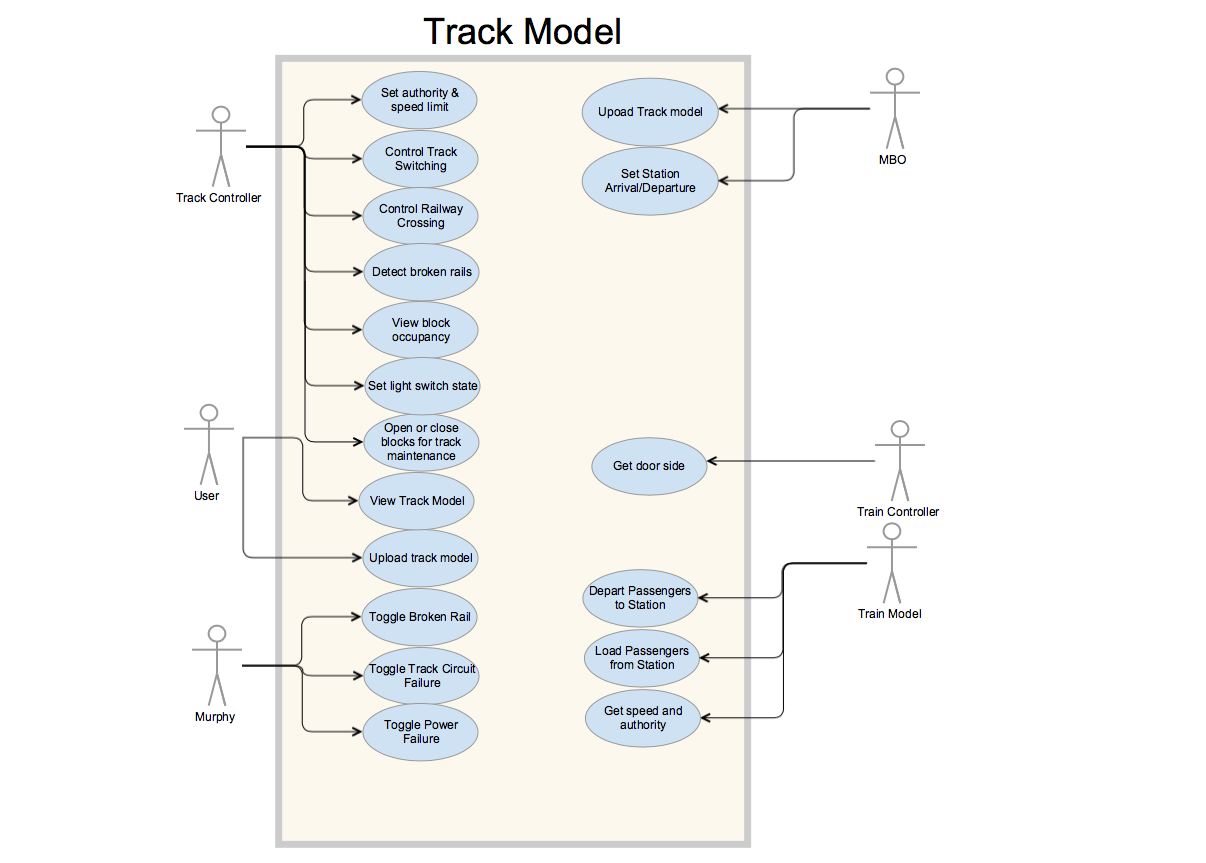
\includegraphics[scale=.15]{trackmodelusecase.png}
	\caption{Track model use case diagram}
\end{figure}

\subsection{Track Controller}
In this subsection, the use cases of the track controller are provided.

\begin{figure}[H]
	\centering
	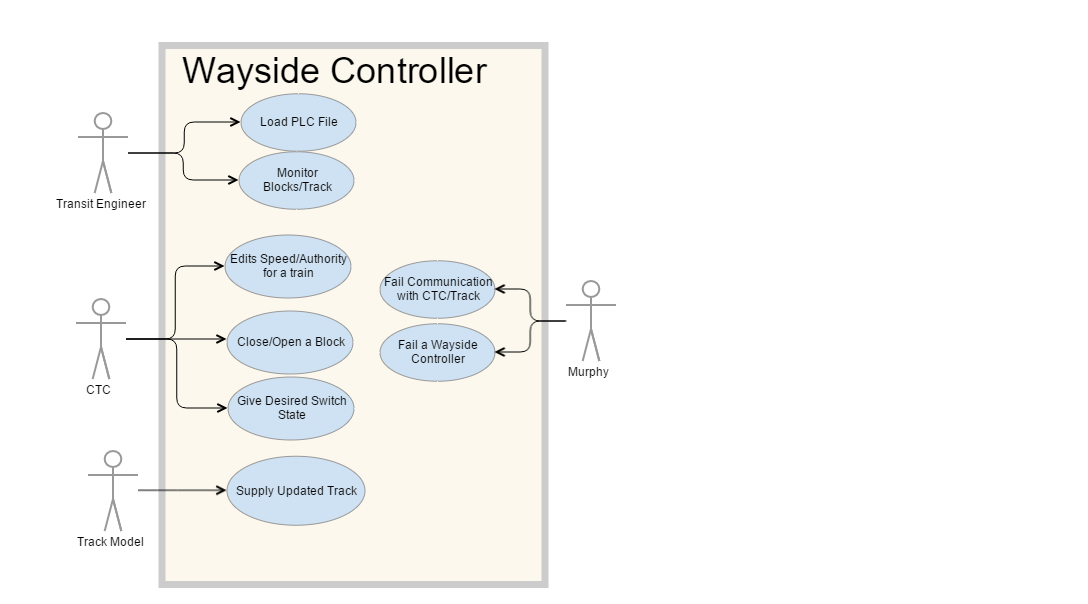
\includegraphics[scale=.2]{trackcontrollerusecase.png}
	\caption{Track controller use case diagram}
\end{figure}

\subsection{Train Model}
In this subsection, the use cases of the train model are provided.

\begin{figure}[H]
	\centering
	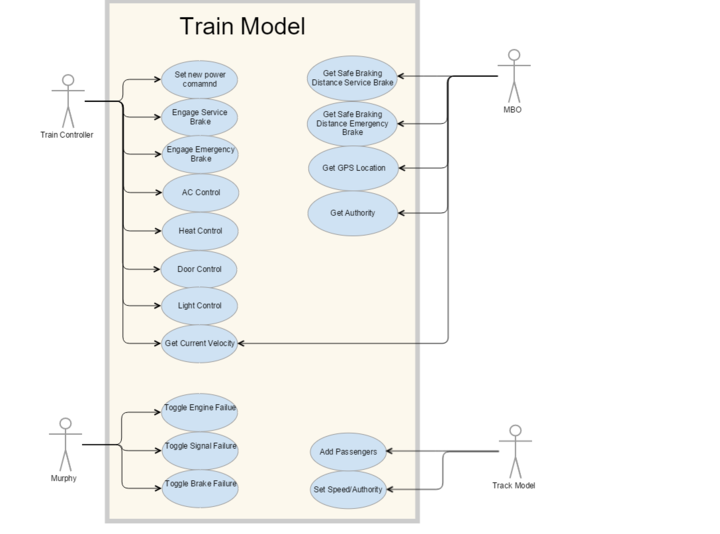
\includegraphics[scale=.2]{trainmodelusecase.png}
	\caption{Train model use case diagram}
\end{figure}

\subsection{Train Controller}
In this subsection, the use cases of the train controller are provided.

\begin{figure}[H]
	\centering
	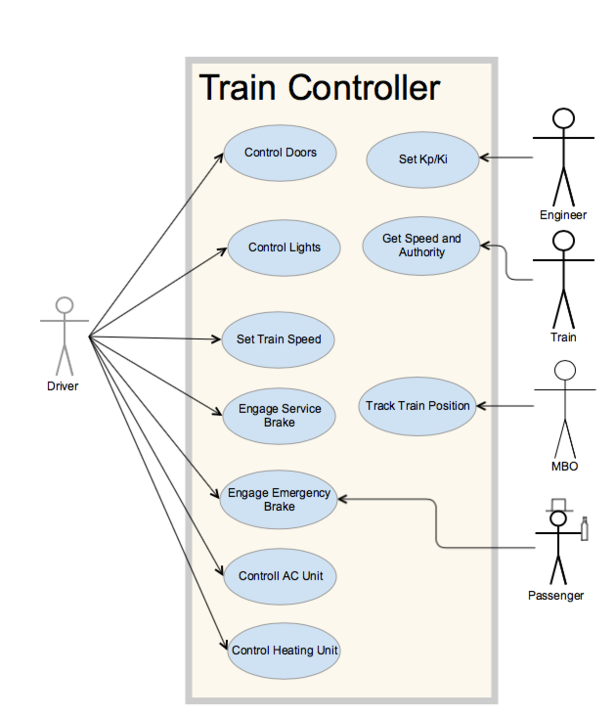
\includegraphics[scale=.2]{traincontrollerusecase.png}
	\caption{Train controller use case diagram}
\end{figure}

\subsection{Moving Block Overlay}
In this subsection, the use cases of the Moving Block Overlay (MBO) are provided.

\begin{figure}[H]
	\centering
	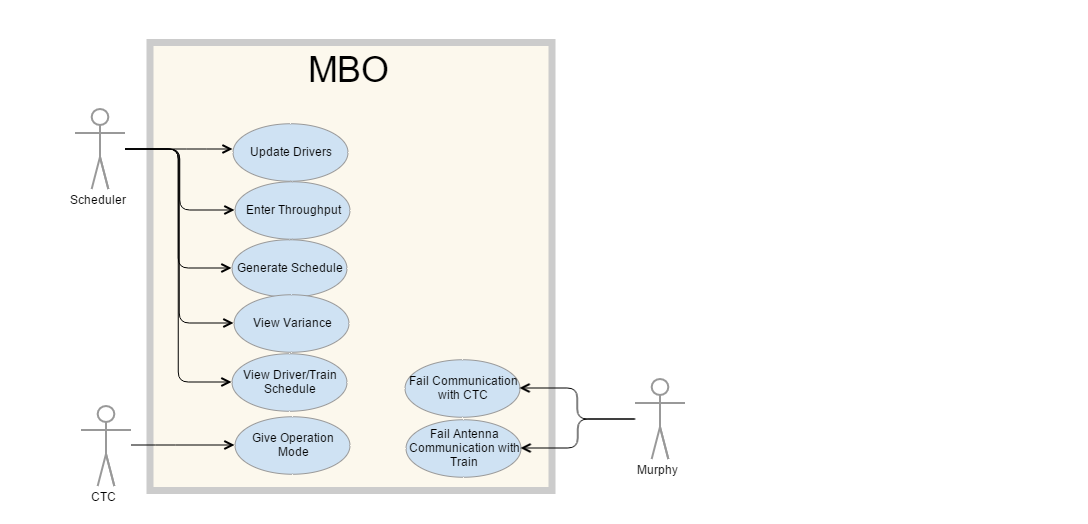
\includegraphics[scale=.2]{mbousecase.png}
	\caption{Train controller use case diagram}
\end{figure}

\subsection{Centralized Train Control}
In this subsection, the use cases of the Centralized Train Control (CTC) are provided.
\begin{figure}[H]
	\centering
	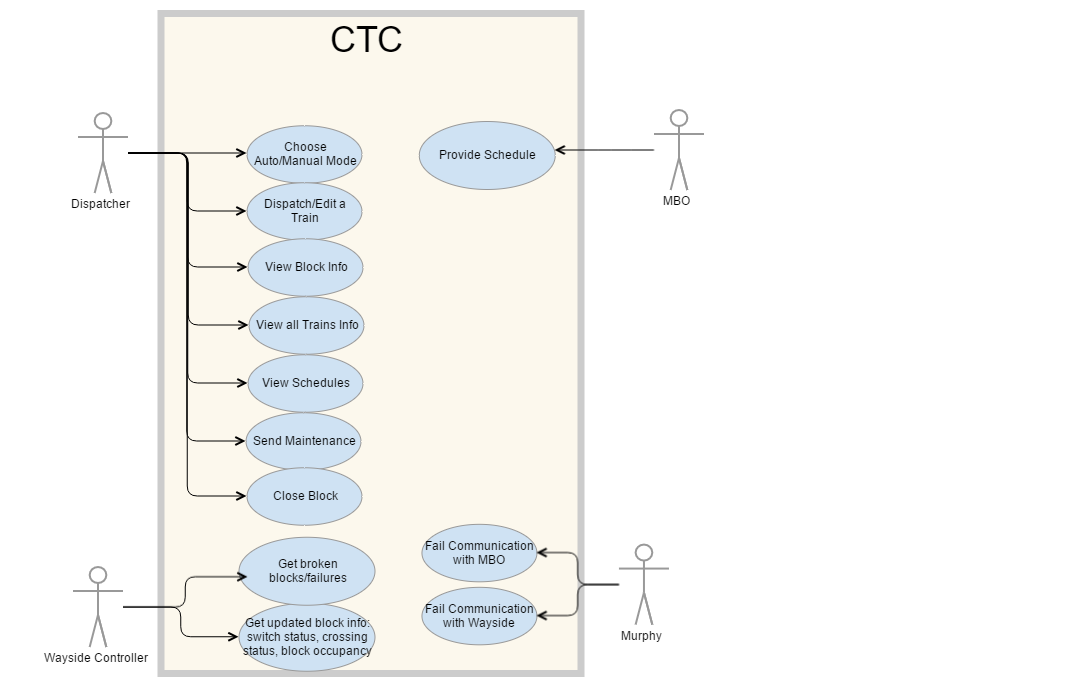
\includegraphics[scale=.15]{ctcusecase.png}
	\caption{Centralized Train Control use case}
\end{figure}

\end{document}          

